% ===================== Appendix E (generated by make_appendix.py) =====================
\section{Numerical illustration}\label{app:experiments}

We illustrate Theorems~\ref{thm:sgda_stability_noA7} and~\ref{thm:pop_excess_risk} on a small MDP in
which every population quantity can be computed exactly. Code and raw results are released with the paper.

\paragraph{Setup.}
The MDP has $|\mathcal S|=5$, $|\mathcal A|=3$, $\beta=0.9$ and $\eta=1$. Rewards are drawn from
$\mathrm{Unif}[0,1]$, and $P(\cdot\mid s,a)=\tfrac12\delta_s+\tfrac12 p_{s,a}$ with
$p_{s,a}\sim\mathrm{Dirichlet}(\mathbf 1)$ (fixed seed). The behaviour policy is uniform, and $\mu$
denotes its stationary state--action distribution (smallest mass $0.046$). We use two data regimes:
(i) $n$ i.i.d.\ transitions with $(s,a)\sim\mu$ and $s'\sim P(\cdot\mid s,a)$; (ii) a single stationary
trajectory of length $n$ under the behaviour policy, whose state chain has second eigenvalue of modulus
$0.59$, so consecutive transitions are dependent. The neighbour $\mathcal D^{(i)}$ replaces a uniformly
chosen $z_i$ by an independent copy $\tilde z_i\sim\mu\otimes P$.

$Q_w$ maps a one-hot state to $|\mathcal A|$ outputs through $H$ softplus units, and $\zeta_v$ maps a
one-hot state--action pair to a scalar through $H$ softplus units, with $H\in\{8,16,32\}$. Both use the
NTK parameterization (output layer scaled by $H^{-1/2}$) with standard Gaussian initialization, and the
output biases start at the constant value scale. Softplus keeps $F_{\mathcal D}$ smooth, as required by
\ref{asm:smooth}. We run Algorithm~\ref{alg:SGDA} with minibatch size $B=32$, stepsizes
$\eta_t=400/(2000+t)$, dual multiplier $\kappa_v=2$ and $T=40{,}000$ iterations, from the same
initialization and with the same minibatch index sequence on $\mathcal D$ and $\mathcal D^{(i)}$. Each
$(n,H)$ pair uses $50$ repetitions, each with a fresh dataset, initialization, index sequence and replaced
index, for $n\in\{100,200,\dots,6400\}$.

We report three quantities: the primal argument stability $\varepsilon^w_T$ of
Theorem~\ref{thm:sgda_stability_noA7}; the function-space distance
$\|Q_{w_T}-Q_{w'_T}\|_{\mu}$; and the excess population MSBE of the output on $\mathcal D$, computed
exactly from $P$. With one-hot inputs both networks can represent any function of their inputs, so
$Q^\star$ is representable and the auxiliary class contains the conditional means; so $\mathcal R(w^\star)=0$ and the excess MSBE equals the left-hand side of
Theorem~\ref{thm:pop_excess_risk}. As a reference we also compute the population MSBE of the exact
empirical minimizer, the fixed point of the empirical soft Bellman operator. Slopes are least-squares fits
of $\log(\text{mean})$ on $\log n$ over $n\ge 200$, with $95\%$ bootstrap intervals over repetitions.

\paragraph{Results.}
Tables~\ref{tab:exp-stability} and~\ref{tab:exp-msbe} and Figure~\ref{fig:exp} report the results. Both
quantities decay as $n^{-1}$: the fitted slopes are between $-1.08$ and $-1.05$ for
$\varepsilon^w_T$ and between $-1.01$ and $-0.97$ for the excess MSBE, every $95\%$ interval
excludes $-1/2$, and $n\,\varepsilon^w_T$ and $n\cdot\mathrm{MSBE}$ stay roughly constant over a $32$-fold
range of $n$. The same holds for a single dependent trajectory (slopes
$-1.01$ and $-0.99$), in line with the fact that
the stability bound needs no independence of the observations. The generalization gap
$\mathcal R(w_T)-\widehat{\mathcal R}_n(w_T)$ of Theorem~\ref{thm:empRM_gen} behaves in the same way
($n$ times the gap lies in $[0.34,0.45]$ for $n\ge200$). No width shows saturation; the
narrowest network has a larger constant but the same rate.

The optimization error is small at $T=40{,}000$: $\varepsilon^w_T$ changes by at most
$15\%$ between $T=20{,}000$ and $T=40{,}000$, and the excess MSBE of
the SGDA output is within $10\%$ of that of the exact empirical minimizer for
$200\le n\le3200$ (within $33\%$ at $n=6400$, where residual optimization error
becomes visible). At $n=100$ some datasets miss a state--action pair, which inflates the error; this point
is excluded from the fits.

\paragraph{Magnitude of the constants.}
For $H=16$ and $n=800$ we estimated the constants along five SGDA trajectories on their own datasets:
$\mu_{\mathrm{PL}}$ and $\rho$ as the smallest observed ratios in \ref{asm:PL-Phi} and \ref{asm:SC},
$\mu_{\mathrm{QG}}$ from \ref{asm:QG-Phi} relative to the final iterate of a run four times longer
(a proxy for the empirical minimizer), $G$ as the largest per-sample gradient norm, and $L$ by power
iteration on the joint Hessian of $F_{\mathcal D}$. Over the whole trajectories the worst values are
$\mu_{\mathrm{PL}}=0.018$, $\rho=0.014$, $\mu_{\mathrm{QG}}=0.012$,
$G=2.5$ and $L=4.2$. With these, the constant $S_w$ of Lemma~\ref{lem:sensitivity}, which multiplies $1/n$
in the primal stability bound, is about $1.0\times10^{5}$, against an observed $n\,\varepsilon^w_T\approx7.3$, and the
statistical constant of Theorem~\ref{thm:pop_excess_risk} is about $3.0\times10^{12}$, against an
observed $n\cdot\mathrm{MSBE}\approx0.41$: with uniform constants the bounds are vacuous at
this scale. The worst values come from early iterates, where the dual variable is far from its maximizer.
Using the median constants after $t=5000$ ($\mu_{\mathrm{PL}}\approx0.95$,
$\rho\approx2.2$, $\mu_{\mathrm{QG}}\approx0.11$) gives $S_w\approx25$,
within a factor of about $3$ of the observed value, while the constant of
Theorem~\ref{thm:pop_excess_risk} (about $1.7\times10^{3}$) remains loose because of its
$(1+L/\rho)^2L_\Phi/(\mu_{\mathrm{PL}}\mu_{\mathrm{QG}})$ dependence. The experiment therefore supports
the $n^{-1}$ rate, not the size of the constants.

\begin{table}[t]
\centering
\footnotesize
\setlength{\tabcolsep}{4pt}
\caption{$n$ times the primal argument stability $\varepsilon^w_T$ (mean $\pm$ standard error over 50
repetitions, $T=40{,}000$). A constant column corresponds to an $n^{-1}$ rate. The last two rows give the
fitted slope of $\log\varepsilon^w_T$ against $\log n$ and its $95\%$ bootstrap interval.}
\label{tab:exp-stability}
\begin{tabular}{@{}rcccc@{}}
\toprule
 & \multicolumn{3}{c}{i.i.d.\ data} & single trajectory \\
\cmidrule(lr){2-4}
$n$ & $H=8$ & $H=16$ & $H=32$ & $H=16$ \\
\midrule
100 & $16.54$ {\scriptsize$\pm2.93$} & $8.95$ {\scriptsize$\pm1.38$} & $5.93$ {\scriptsize$\pm0.65$} & $9.93$ {\scriptsize$\pm1.20$} \\
200 & $11.88$ {\scriptsize$\pm1.33$} & $7.74$ {\scriptsize$\pm0.57$} & $7.18$ {\scriptsize$\pm0.61$} & $7.70$ {\scriptsize$\pm1.06$} \\
400 & $13.13$ {\scriptsize$\pm2.93$} & $8.38$ {\scriptsize$\pm0.78$} & $7.39$ {\scriptsize$\pm0.65$} & $6.77$ {\scriptsize$\pm0.55$} \\
800 & $8.45$ {\scriptsize$\pm0.56$} & $6.72$ {\scriptsize$\pm0.59$} & $6.27$ {\scriptsize$\pm0.44$} & $6.58$ {\scriptsize$\pm0.68$} \\
1600 & $8.84$ {\scriptsize$\pm0.73$} & $6.95$ {\scriptsize$\pm0.62$} & $5.59$ {\scriptsize$\pm0.55$} & $7.20$ {\scriptsize$\pm0.53$} \\
3200 & $10.32$ {\scriptsize$\pm1.14$} & $7.65$ {\scriptsize$\pm0.70$} & $5.75$ {\scriptsize$\pm0.48$} & $7.40$ {\scriptsize$\pm0.85$} \\
6400 & $9.03$ {\scriptsize$\pm0.77$} & $6.33$ {\scriptsize$\pm0.66$} & $6.05$ {\scriptsize$\pm0.54$} & $6.86$ {\scriptsize$\pm0.74$} \\
\midrule
slope ($n\ge 200$) & $-1.08$ & $-1.05$ & $-1.07$ & $-1.01$ \\
95\% interval & {\scriptsize$[-1.16,-1.00]$} & {\scriptsize$[-1.11,-0.99]$} & {\scriptsize$[-1.13,-1.01]$} & {\scriptsize$[-1.09,-0.93]$} \\
\bottomrule
\end{tabular}
\end{table}

\begin{table}[t]
\centering
\footnotesize
\setlength{\tabcolsep}{4pt}
\caption{$n$ times the excess population MSBE of the SGDA output (mean $\pm$ standard error), and of the
exact empirical minimizer on the datasets of the i.i.d.\ $H=16$ runs.}
\label{tab:exp-msbe}
\begin{tabular}{@{}rccccc@{}}
\toprule
 & \multicolumn{3}{c}{i.i.d.\ data} & single trajectory & exact empirical \\
\cmidrule(lr){2-4}
$n$ & $H=8$ & $H=16$ & $H=32$ & $H=16$ & minimizer (i.i.d.) \\
\midrule
100 & $0.480$ {\scriptsize$\pm0.035$} & $0.834$ {\scriptsize$\pm0.127$} & $0.508$ {\scriptsize$\pm0.036$} & $0.819$ {\scriptsize$\pm0.274$} & $0.672$ \\
200 & $0.457$ {\scriptsize$\pm0.031$} & $0.440$ {\scriptsize$\pm0.039$} & $0.448$ {\scriptsize$\pm0.025$} & $0.461$ {\scriptsize$\pm0.038$} & $0.436$ \\
400 & $0.447$ {\scriptsize$\pm0.037$} & $0.393$ {\scriptsize$\pm0.020$} & $0.446$ {\scriptsize$\pm0.025$} & $0.411$ {\scriptsize$\pm0.026$} & $0.391$ \\
800 & $0.420$ {\scriptsize$\pm0.026$} & $0.412$ {\scriptsize$\pm0.022$} & $0.391$ {\scriptsize$\pm0.021$} & $0.430$ {\scriptsize$\pm0.029$} & $0.404$ \\
1600 & $0.433$ {\scriptsize$\pm0.029$} & $0.385$ {\scriptsize$\pm0.020$} & $0.383$ {\scriptsize$\pm0.020$} & $0.375$ {\scriptsize$\pm0.022$} & $0.358$ \\
3200 & $0.464$ {\scriptsize$\pm0.029$} & $0.396$ {\scriptsize$\pm0.024$} & $0.414$ {\scriptsize$\pm0.025$} & $0.429$ {\scriptsize$\pm0.029$} & $0.361$ \\
6400 & $0.527$ {\scriptsize$\pm0.033$} & $0.443$ {\scriptsize$\pm0.026$} & $0.455$ {\scriptsize$\pm0.022$} & $0.486$ {\scriptsize$\pm0.023$} & $0.350$ \\
\midrule
slope ($n\ge 200$) & $-0.97$ & $-1.00$ & $-1.01$ & $-0.99$ & $-1.06$ \\
95\% interval & {\scriptsize$[-1.01,-0.92]$} & {\scriptsize$[-1.05,-0.95]$} & {\scriptsize$[-1.04,-0.97]$} & {\scriptsize$[-1.03,-0.94]$} & {\scriptsize$[-1.11,-1.02]$} \\
\bottomrule
\end{tabular}
\end{table}

\begin{figure}[t]
\centering
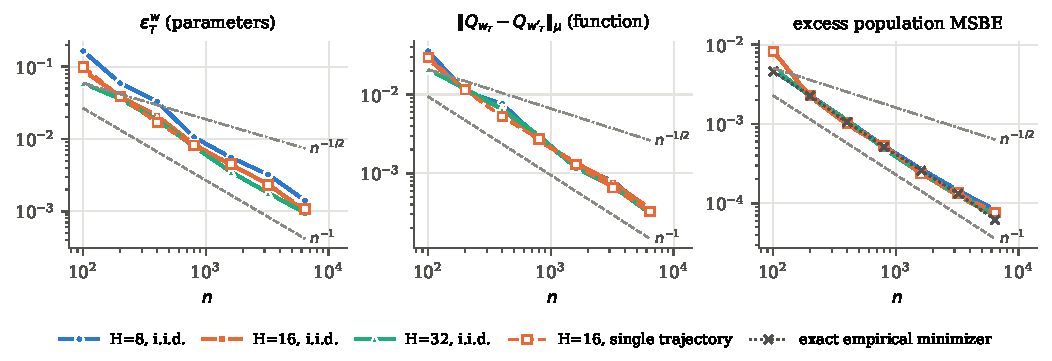
\includegraphics[width=\textwidth]{stability_vs_n.pdf}
\caption{Primal argument stability, function-space stability and excess population MSBE against $n$
(log--log). Solid lines: i.i.d.\ data; dashed: a single trajectory. Grey guides show slopes $-1$ and
$-1/2$.}
\label{fig:exp}
\end{figure}
